\paragraph{QuizziPedia::Front-End::Directives::SearchDirective}

\label{QuizziPedia::Front-End::Directives::SearchDirective}

\begin{figure}[h]
	\centering
	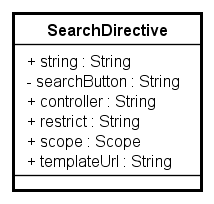
\includegraphics[scale=0.5,keepaspectratio]{UML/Classi/Front-End/QuizziPedia_Front-end_Directives_SearchDirective.png}
	\caption{QuizziPedia::Front-End::Directives::SearchDirective}
\end{figure}

\begin{itemize}
	\item \textbf{Descrizione}: directive che permette di effettuare la ricerca di utenti e questionari;
	\item \textbf{Utilizzo}: permette all'utente di effettuare ricerche, è strutturata da:
	\begin{itemize}
		\item Barra di ricerca;
		\item Pulsante per effettuare la ricerca;
	\end{itemize}
	\item \textbf{Relazioni con altre classi}:
	\begin{itemize}
			\item \textit{IN} \texttt{HomeView} 
		\item \textit{IN} \texttt{MenuBarDirective} 
	\end{itemize}
	\item \textbf{Attributi}
\end{itemize}

\paragraph{QuizziPedia::Front-End::Directives::StatisticsDirective}

\label{QuizziPedia::Front-End::Directives::StatisticsDirective}

\begin{figure}[h]
	\centering
	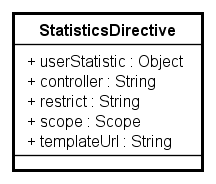
\includegraphics[scale=0.5,keepaspectratio]{UML/Classi/Front-End/QuizziPedia_Front-end_Directives_StatisticsDirective.png}
	\caption{QuizziPedia::Front-End::Directives::StatisticsDirective}
\end{figure}

\begin{itemize}
	\item \textbf{Descrizione}: directive che permette di visualizzare le statistiche di un utente;
	\item \textbf{Utilizzo}: permette di visualizzare le statistiche, in particolare viene utilizzata per mostrare statistiche:
	\begin{itemize}
		\item Nella pagina della visualizzazione del profilo;
		\item Di un utente ricercato tramite apposita funzione.
	\end{itemize}
	\item \textbf{Relazioni con altre classi}:
	\begin{itemize}
		\item \textit{IN} \texttt{UserView} 
		\item \textit{IN} \texttt{OtherUserView} 
		\item \textit{OUT} \texttt{StatisticsController} 
	\end{itemize}
	\item \textbf{Attributi}
\end{itemize}

\paragraph{QuizziPedia::Front-End::Directives::SubscribeResultDirective }

\label{QuizziPedia::Front-End::Directives::SubscribeResultDirective}

\begin{figure}[h]
	\centering
	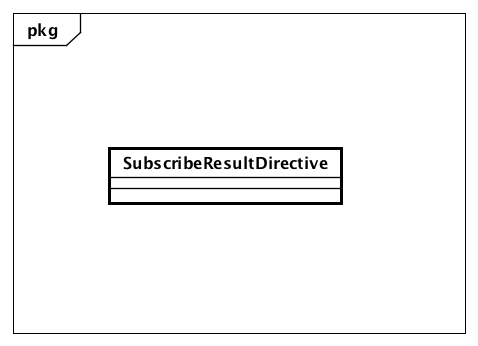
\includegraphics[scale=0.5,keepaspectratio]{UML/Classi/Front-End/QuizziPedia_Front-end_Directives_SubscribeResultDirective.png}
	\caption{QuizziPedia::Front-End::Directives::SubscribeResultDirective}
\end{figure}

\begin{itemize}
	\item \textbf{Descrizione}: directive che permette di visualizzare e iscriversi ai questionari ricercati;
	\item \textbf{Utilizzo}: permette di visualizzare e iscriversi ai questionari ricercati. Include un pulsate per ogni questionario che permette l'iscrizione ad esso.
	\item \textbf{Relazioni con altre classi}:
	\begin{itemize}
		\item \textit{IN} \texttt{ResultsView} 
	\end{itemize}
	\item \textbf{Attributi}
\end{itemize}

\paragraph{QuizziPedia::Front-End::Directives::TopicKeywordsDirective}

\label{QuizziPedia::Front-End::Directives::TopicKeywordsDirective}

\begin{figure}[h]
	\centering
	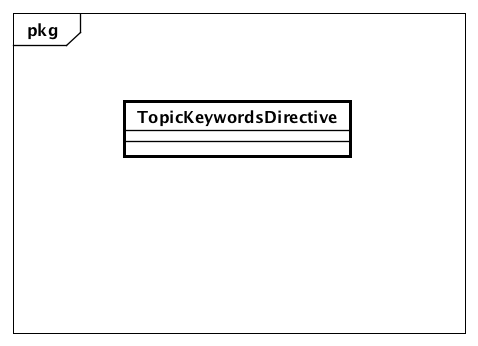
\includegraphics[scale=0.5,keepaspectratio]{UML/Classi/Front-End/QuizziPedia_Front-end_Directives_TopicKeywordsDirective.png}
	\caption{QuizziPedia::Front-End::Directives::TopicKeywordsDirective}
\end{figure}

\begin{itemize}
	\item \textbf{Descrizione}: directive che permette di gestire l'inserimento di keywords al momento della creazione della domanda;
	\item \textbf{Utilizzo}: permette l'inserimento di keywords al momento di creazione della domanda, in particolare sarà formata da:
	\begin{itemize}
		\item Un menù a tendina per selezionare l'argomento della domanda;
		\item Un campo di testo in cui inserire le keywords.
	\end{itemize}
	\item \textbf{Relazioni con altre classi}:
	\begin{itemize}
		\item \textit{IN} \texttt{TrueFalseQuestionsView} 
		\item \textit{IN} \texttt{MultiplyQuestionsView} 
		\item \textit{IN} \texttt{ConnectionQuestionsView}
		\item \textit{IN} \texttt{ImagesSortingQuestionsView} 
		\item \textit{IN} \texttt{StringsSortingQuestionsView} 
		\item \textit{IN} \texttt{FillingQuestionsView} 
		\item \textit{IN} \texttt{ClickableAreaQuestionsView} 
		\item \textit{IN} \texttt{EditorQMLView} 
	\end{itemize}
	\item \textbf{Attributi}
\end{itemize}

\paragraph{QuizziPedia::Front-End::Directives::UserDetailsDirective}

\label{QuizziPedia::Front-End::Directives::UserDetailsDirective}

\begin{figure}[h]
	\centering
	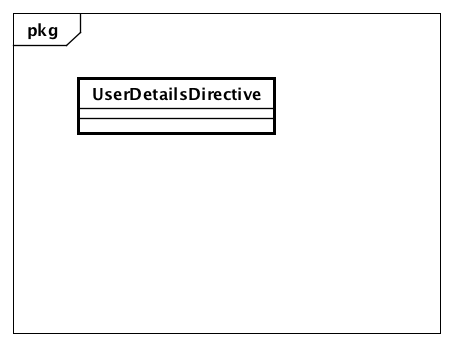
\includegraphics[scale=0.5,keepaspectratio]{UML/Classi/Front-End/QuizziPedia_Front-end_Directives_UserDetailsDirective.png}
	\caption{QuizziPedia::Front-End::Directives::UserDetailsDirective}
\end{figure}

\begin{itemize}
	\item \textbf{Descrizione}: directive che permette di visualizzare i dati personali di un utente;
	\item \textbf{Utilizzo}: permette di visualizzare i dati personali di un utente, in dettaglio conterrà:
	\begin{itemize}
		\item Nome;
		\item Cognome;
		\item Email.
	\end{itemize}
	\item \textbf{Relazioni con altre classi}:
	\begin{itemize}
		\item \textit{IN} \texttt{UserView} 
		\item \textit{OUT} \texttt{UserDetailsController} 
	\end{itemize}
	\item \textbf{Attributi}
\end{itemize}

\paragraph{QuizziPedia::Front-End::Directives::UserResultsDirective}

\label{QuizziPedia::Front-End::Directives::UserResultsDirective}

\begin{figure}[h]
	\centering
	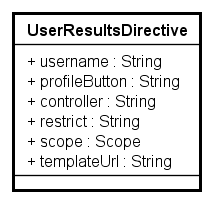
\includegraphics[scale=0.5,keepaspectratio]{UML/Classi/Front-End/QuizziPedia_Front-end_Directives_UserResultsDirective.png}
	\caption{QuizziPedia::Front-End::Directives::UserResultsDirective}
\end{figure}

\begin{itemize}
	\item \textbf{Descrizione}: directive che permette di visualizzare la lista degli utenti ricercati dopo aver utilizzato l'apposita funzione di ricerca;
	\item \textbf{Utilizzo}: permette di visualizzare la lista degli utenti, in particolare conterrà:
	\begin{itemize}
		\item Nome dell'utente;
		\item Pulsante per poter essere reindirizzati alla pagina di visualizzazione del profilo dell'utente selezionato.
	\end{itemize}
	\item \textbf{Relazioni con altre classi}:
	\begin{itemize}
		\item \textit{IN} \texttt{ResultsView} 
	\end{itemize}
	\item \textbf{Attributi}
\end{itemize}
